\documentclass[a4paper]{article}
\usepackage[right=1in, left=1in, top=1in, bottom=1in]{geometry}
\usepackage{graphicx}
\begin{document}
	\title{\textbf{MACHINE LEARNING LAB}}
	\maketitle
	\centering{\textbf{Manish Singh CS3}\\[2.5]\\}
	\centering{\textbf{Roll No. 17/466}\\[2.5]\\}
	\begin{figure}[h]
		\centering
		
\includegraphics{rtu.jpeg}
	\end{figure}
	\begin{large}
		\\Computer Science and Engineering Department\\
	\end{large}\\
	\textit{\begin{Large}
			\\Rajasthan Technical University, Kota\\
	\end{Large}}
	\newpage
	\flushleft
	\tableofcontents
	\newpage
	\section{Problem Statement}
	Implement and demonstrate the FIND-S algorithm for finding the most specific hypothesis based on a given set of training data samples. Read the training data samples from a .CSV file.(enjoysport.csv)\\
	\section{FIND-S algorithm}
	1. Initialize $h$ to the most specific hypothesis in $H$\\
	2. For each positive training instance $x$\\
	\hspace{10mm}For each attribute constraint $a_i$ in $h$\\
	\hspace{20mm}If the constraint $a_i$ is satisfied by $x$\\
	\hspace{20mm}Then do nothing\\
	\hspace{20mm}Else replace $a_i$ in $h$ by the next more general constraint that is satisfied by $x$\\
	
	3. Output hypothesis $h$
	\\\
	\\
	\\
	\\
	
	\section{Training Set}
	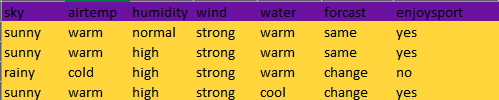
\includegraphics[scale=1.3]{enjoysport.png}\\
	\\
	\\
	\newpage
	\section{Program}
	\begin{verbatim}
		import pandas as pd
	
	df = pd.read_csv("enjoysport.csv")
	print("The data is: \n\n",df)
	print("\n"+"*" * 70)
	print("The shape of dataset is",df.shape,"\n")
	# defining the attributes
	num_attributes = 6
	#initialize the instance
	a = []
	#stroing the dataset items in list
	for i in range(len(df)):
	a.append(df.iloc[i].tolist())
	
	#storing zero at every place 
	hypo = ['0']* num_attributes
	# initialize the specific hypothesis
	for j in range(0, num_attributes):
	hypo[j] = a[0][j]
	print("Most Specific hypotheis is: ",hypo)
	# For each positive training instance x
	for i in range(len(a)):
	if a[i][num_attributes]=='yes':
	for j in range(0,num_attributes):# For each attribute constraint ai in h
	if a[i][j] != hypo[j]:# Else replace ai in h by the next more general constraint that is satisfied by x
	hypo[j]="?"
	else:# If the constraint ai is satisfied by x
	hypo[j]=a[i][j]# Then do nothing
	print(" \n\nFor Training instance No:{0} the hypothesis is\n".format(i),hypo)    # Output hypothesis h       
	
	print("\n The Maximally Specific Hypothesis for a given Training Examples :\n")
	print(hypo)
	\end{verbatim}
	\section{Output}
	\fbox{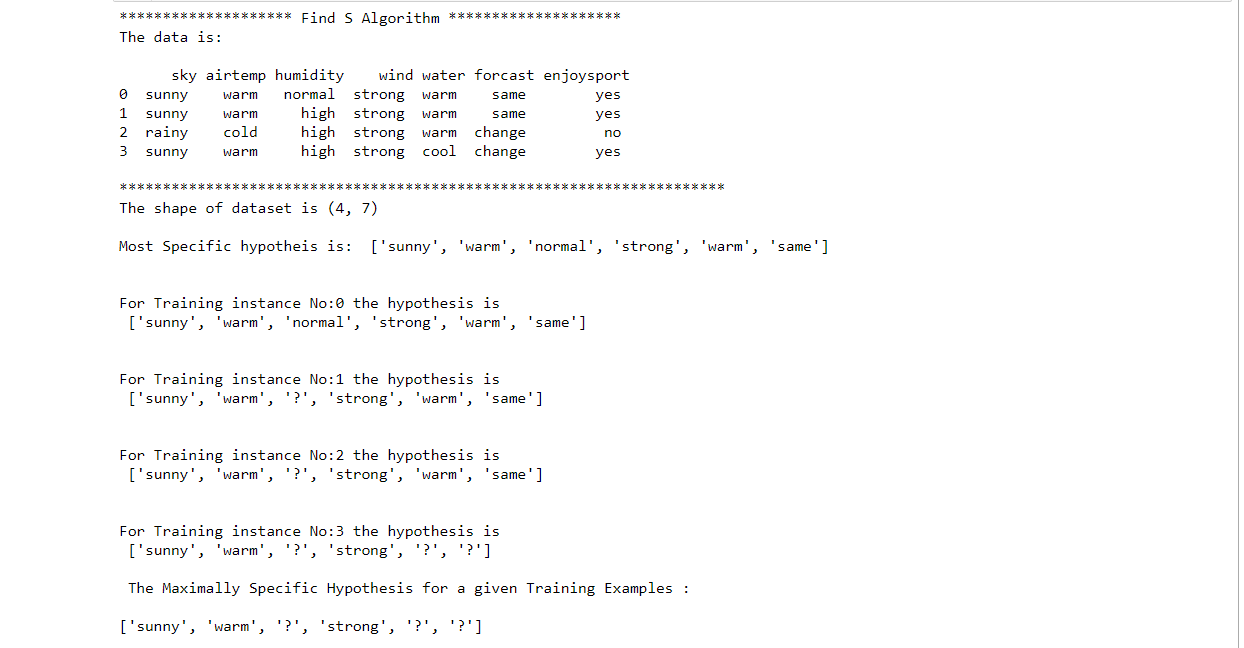
\includegraphics[scale=1.0]{finds.png}}
	\section{Result}
	We have found the most specific hypothesis based on a given set of training data samples using FIND-S algorithm.
\end{document}